\documentclass[9pt,b5j,papersize]{jsarticle}
\usepackage[dvipdfmx]{graphicx}
\usepackage{wrapfig}
\usepackage{float}
\usepackage{otf}
\usepackage{longtable}
\usepackage{ulem}
\usepackage{ascmac}
\usepackage{titlesec}
\usepackage{multicol}
%%%脚注を文末に出す
\usepackage{endnotes}
\let\footnote=\endnote
\renewcommand{\theendnote}{\arabic{endnote})}
\renewcommand{\notesname}{{\small 註}}
\def\ennotesize{\normalsize}
\def\notessize{\normalsize}
\usepackage{etoolbox}
\patchcmd{\enoteformat}{1.8em}{0pt}{}{}
%%%
\setlength{\textwidth}{150truemm}      % テキスト幅: 160mm
\setlength{\fullwidth}{\textwidth}     % ページ全体の幅
\setlength{\oddsidemargin}{-10truemm}   % 左余白
\setlength{\topmargin}{-10truemm}       % 上余白
\setlength{\textheight}{210truemm}     % テキスト高さ: 297-(30+30)=237mm
\pagestyle{empty}
%%%文字数と行数を指定する
\makeatletter
\def\mojiparline#1{
    \newcounter{mpl}
    \setcounter{mpl}{#1}
    \@tempdima=\linewidth
    \advance\@tempdima by-\value{mpl}zw
    \addtocounter{mpl}{-1}
    \divide\@tempdima by \value{mpl}
    \advance\kanjiskip by\@tempdima
    \advance\parindent by\@tempdima
}
\makeatother
\def\linesparpage#1{
    \baselineskip=\textheight
    \divide\baselineskip by #1
}
%%%見出しの表示方法変更
%\titleformat*{\section}{\large\bfseries\textgt}
%\titleformat*{\subsection}{\normalsize\bfseries\textgt}{\filright(\,\thesubsection\,)}
%%%

\begin{document}
% 1行あたりの文字数指定
\mojiparline{48}
% 1ページあたり行数の指定
\linesparpage{44}
%%%%%%%%%%%%%%%%

\begin{center}
{\huge 考古学情報の再現可能性}

\vspace{1\baselineskip}
{\Large 〜バージョン管理システムGitを利用した調査データの管理と公開〜}
\end{center}

\vspace{3\baselineskip}

\begin{flushright} {\large 石井淳平} \end{flushright}

\vspace{1\baselineskip}

\begin{multicols}{2}

%%%%
\noindent
{\large はじめに}

発掘調査記録をオープンデータとして活用するための方策として、GitHubに代表されるバージョン管理+共有サービスを利用した考古学情報の管理と共有について考える。図書として刊行された発掘調査報告書は、情報の固定という面で優れているが、報告書作成に利用された調査記録や中間成果物へのアクセシビリティが低く、再現性が低いことが問題である。このことは、考古学情報の真正性の問題ともかかわるとともに、考古学情報の社会的利用の根幹に関わる問題である。こうした課題を解決する手法としてバージョン管理システムGitの利用を提案する。

Gitを使用し、一次情報である現場図面や写真、最終的な報告書に至る中間成果物すべての改変履歴を記録することで考古学情報の真正性と再現可能性が担保される。また、Gitの機能を利用したウェブサービスであるGitHubにより考古学情報の作成に関わった調査記録の公開が実現する。本報告では、北海道南部の箱館戦争遺跡の調査においてGitによるバージョン管理とGitHubを利用したデータ共有の実践例を紹介し、手法やノウハウを報告する。

%%%%
\noindent
{\large 1.ブラックボックス化する考古学情報}

考古学情報の保存・公開に用いられる媒体については、紙でもPDFでも情報の再現可能性としては同質である。考古学情報の公開にあたって解決しなければならないのは発掘調査報告のブラックボックス化である。筆者は考古学情報を再利用可能なデータ群として流通させることが考古学における情報化の最大の課題と捉えている。

発掘調査報告書の作成には現地で作成した図面、撮影された写真、測量記録などの一次情報のほかに、それらを整理・清書した中間的な二次情報がある。例えば、最終的に報告書に掲載される遺物集計表は遺物の整理分類に使用された「遺物台帳」を元に作成されている。しかし、最終的な報告書しか手にすることができない者にはこれらの集計作業が適切に行われたかどうかを判断するすべはない。

また、現地で作成した平面図と断面図には必ず誤差が生じる。多くの場合、「素図」や「第二原図」などと呼ばれる清書図面を作成する際に、原図の修正作業が行われる。どのような修正が行われたのか、その修正は適切だったのかを第三者が知ることはできない。

こうした「修正」作業は限度を超えると「捏造」と変わらない。測量では誤差を全体に散らして、総合的な誤差を「閉合誤差」のように定量化するが、たとえば遺構計測の際にそのような取り扱いがなされているケースを筆者は知らない。修正の履歴を残すことが考古学情報の再現可能性を高めることにつながる。

%%%%
\noindent
{\large 2.考古学情報の「真正性」}

要するに、考古学情報の再現可能性を高めることは、考古学情報の「真正性」を高めることにほかならない。考古学情報の「真正性」を文化財における「真正性(authenticity)」に引きつけて表現すると次のとおりである。

\begin{itemize}
\item 考古学情報の価値は真正性によって評価される
\item そのためには考古学情報の作成に使用された情報源が信頼できる度合いが評価されなければならない
\item どのようなプロセスで考古学情報が作成されたのかに関する情報が真正性の評価には必須である
\end{itemize}

つまり考古学情報作成プロセスを明示することが、考古学情報の真正性を評価するための第一歩となる。どのように調査記録が選択され、どのような処理を経て最終的な考古学情報として成立したのかという点に関するメタデータの存在こそが考古学情報の真正性を評価する基本となる。

%%%%
\noindent
{\large 3.データの長期保存とともに考えるべきこと}

「真正性」という視点で考古学情報を考えたとき、単なる調査記録の長期保存を考えるだけでは不十分だということになる。真正性を評価するためには、より上位の情報として「考古学情報作成プロセスとしての調査記録の新設・追加・変更の履歴」が必要となる。これは考古学情報の再現にかかるメタ情報であり、第三者が報告書を再構築できる情報であることが求められる。



%%%%
\noindent
{\large 4.Gitを利用した発掘調査記録管理}

筆者がイメージする発掘調査記録管理のイメージにもっとも近いのはGitを使ったバージョン管理とGitHubによるデータ共有である。Gitの適切な使用によって、「どのような改変が」、「いつ」、「誰によって」行われたのかが明示的になる。GitHubのようなデータ共有環境を利用することで、Gitによってバージョン管理されたデータ群を、誰でも利用できるようになる。

Git本体の主な機能は情報の変更単位
\footnote{Gitにおける一種の「保存」作業で、「commit」という操作によって特定のディレクトリに対してなされた変更が記録される}
ごとに履歴を作成するものである。任意のタイミングで変更をGitに登録することができる。Gitによる変更履歴の登録には次のようなメリットがある。

いつ、どのような変更が、誰によって行われたのかが明確になる。報告書作成作業では、現場図面をトレースして掲載図版を作成する。このとき、調査者によって不要と判断された記録は掲載図版には転記されない。また、現場図面には記載のない調査担当者の野帳の情報が掲載図版に転記されることもある。上面写真の情報を掲載図版に付記する場合もある。最終的な成果に記載された情報が、どの時点で、誰によって付加されたのかがGitによって明確になる。

過去に遡って記録を回収できる。報告書作成作業では日々の作業で次々と記録が更新されていく。通常、上書きされ、消去された記録を復元することは難しい。仮にバックアップ機能などで記録の復元を行ったとしても、復元された記録が、変更履歴全体の中で整合性を保つことは難しくなる。Gitでは変更単位ごとに全ての変更が記録されているため、消去、改変された過去の記録を復元し、取り出すことが可能となる。このことは、記録を「念の為に保存しておく」という行為を不要にし、最終的な考古学情報にノイズが含まれることを防ぐとともに、中間成果物も維持されるため、結果的に考古学情報作成にかかわる全ての記録が保存されることとなる。

%%%%
\noindent
{\large 5.Git利用の実際}

Gitはコマンドラインで操作されることが多く、筆者も基本的にはコマンドラインでGitを操作している。原稿執筆環境がテキストエディタ中心であることから、別途Git用のアプリケーションを起動することなく執筆作業に集中できること、日常的に使用するGitコマンドがシンプルで暗記しやすいためである。

ただし、Gitには秀逸なGUIクライアントソフトが数多く開発されており(GitKraken、GitCola、SourceTreeなど)、これらのソフトウェアによりGitを操作することが可能である。筆者はシンプルなGitColaをインストールしている。GUIクライアントソフトを利用することでコマンド入力から解放されること、変更履歴(commitという)や変更の分岐(branch)や結合(merge)が視覚的に一覧できるメリットがある。

Gitでの基本的な作業は「commit」と呼ばれる変更履歴の登録である。特定のディレクトリ(例えば発掘調査報告書作成用のディレクトリ)に対して行われた変更の全てが「commit」を行うことでGitのリポジトリ(データベースのようなもの)に登録される。「commit」の際に適切なコメント(「F2塹壕図のグリッドラインを描画し、断面を修正」など)を付すことで変更の内容が第三者にもわかるようになる。

GitHubなどのウェブでの共有サービスを利用している場合は「Push」という操作が必要になる。これは最新の変更をGitHubに反映させるためのものである。

別の編集者がGitHubにあるデータに対して変更を加えた場合には「Pull」という操作で変更点をダウンロードし、自分のコンピュータとGitHubのデータを同期する。

以上をまとめるとGit及びGitHubを利用したデータ共有は「Pull」コマンドでGitHubと自分のPCを同期し、「commit」で変更内容を登録する。最後に「Push」で自分が加えた変更をGitHubに反映させる、という三段階によって自分を含めた執筆者のPC内のデータとGitHubのデータが一致している状態が保たれる。


%%%%
\noindent
{\large 6.北海道北斗市二股台場調査でのGit利用}

筆者らが取り組んでいる北海道南西部北斗市二股台場の測量調査では、GitHubによる調査記録の公開(https://github.com/IshiiJunpei/Futamata)を行っている。

本調査は「箱館戦争遺跡プロジェクト」という有志が主体となって実施しているものであり、関係者が日常的に顔をあわせて作業する環境にはない。そのため、調査情報をリモートで共有する必要があったこと、複数の調査者が調査記録の編集に関わることから、作業重複を避ける工夫が必要であった。調査ではGitとGitの仕組みを利用したGitHubというウェブサービスを利用して調査記録更新にかかる公正性の確保と作業重複の回避を行った。

複数の調査者で調査記録を共有する際に重要なことは適切なディレクトリ構造とファイル名付与である。考古学記録のアーカイブ方法については愛知県埋蔵文化財センターの電子納品ガイドラインが先行的な取り組みといえる(堀木2018)。二股台場調査では筆者の扱いやすいディレクトリ構造やファイル名付与を行ったが、標準化されるべきことがらの一つであろう。

\begin{figure}[H]
\centering
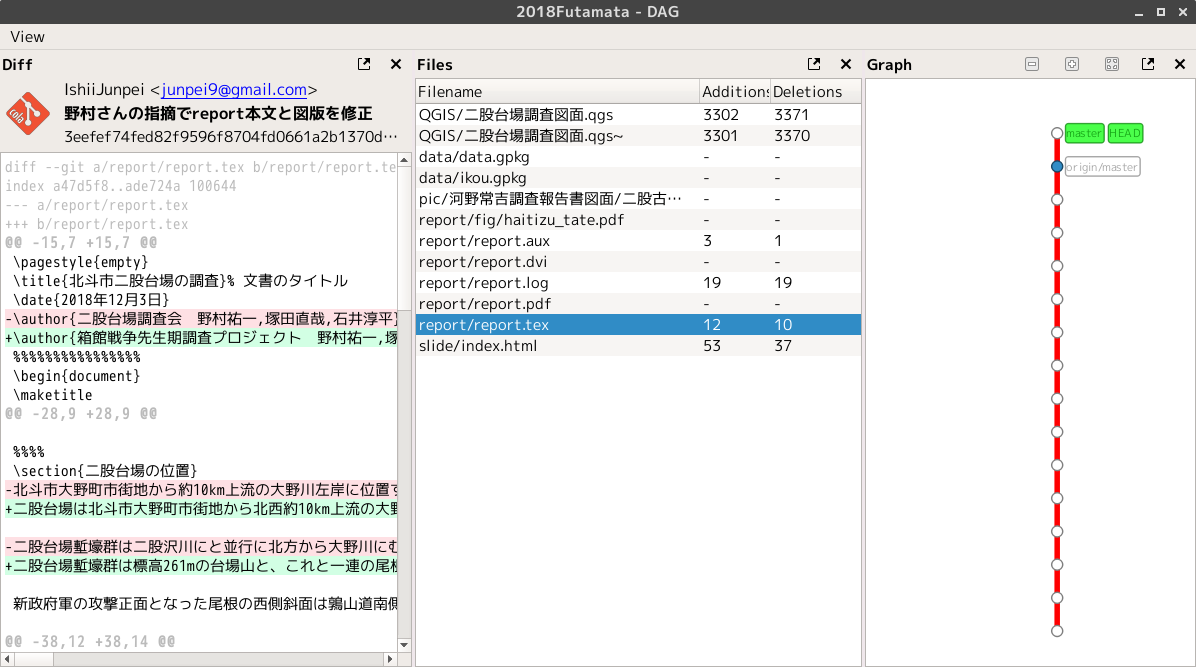
\includegraphics[width=1\linewidth]{01.png}
\caption{二股台場調査のGit情報}
\label{hutamata}
\end{figure}

図\ref{hutamata}は二股台場調査記録のログである。右のペインはGitの更新履歴を示す。中央ペインは変更が行われたファイルの一覧である。変更が行われたファイルを選択すると左ペインにファイルの内容と変更箇所が示される。共同調査者からの指摘で報告文本文の修正と図版データの修正を行った変更ログである。このように全ての変更履歴が変更後の差分とあわせて確認できることがGitを利用する大きなメリットとなる。


%%%%
\noindent
{\large 7.コンパイル状態の考古学情報}

図書として刊行された考古学情報は一種のコンパイル状態といえる。「コンパイル」とは、プログラミングコードをコンピュータが読むための2進法の記号に変換することであり、コンパイルされたプログラムは人間が読むことはできない。コンパイル状態の情報は真偽を問うことも、ソースを再利用することも不可能である。

紙媒体やPDF保存された発掘調査報告書も中身の情報の真偽を問うことやデータを再利用することが不可能という点でコンパイルされた状態といえる。コンパイル状態の報告書からは最終的な結果を知ることができても、元になった調査記録や中間成果物などの再利用可能なデータを取り出すことは不可能である。


%%%%
\noindent
{\large 8.オープンデータとしての考古学情報}

考古学情報が適切なデータを使用して作成されているか、適切な手順を踏んで作成されているかを判断するためには、ソースコードに相当する調査記録や中間成果物にアクセスできる環境が必要となる。考古学情報の真正性は「情報の固定化(コンパイル化)」ではなく、すべての情報に市民がアクセスできる環境の構築によって担保される、というのが筆者の考え方だ。

オープンソースのソフトウェアのソースコードから必要な部分を切り取って自由に利用できるようになったことで、コンピュータソフトウェアの開発が大きく進んだのと同じように、考古学情報にかかわる調査記録や中間成果物を自由に利用できるようになる学問上のメリットははかりしれない。

全国遺跡報告総覧への報告書アップロードも十分とは言えない状態であり、筆者のアイディアは時期尚早といえるかもしれないが、自らの研究環境を向上させるための工夫を続けるという地道な取り組み以外に変化を起こす方法はないと信じている。


\vspace{1\baselineskip}
\noindent
引用参考文献\\
堀木真美子 2018「発掘調査データの整理と公開システム」『文化財の壺』Vol.6,文化財方法論研究会,pp.8-11
\end{multicols}{2}
\end{document}
